\documentclass[tikz,border=3mm]{standalone}
\usetikzlibrary{arrows.meta,calc,positioning}
\begin{document}
\pagecolor{white}
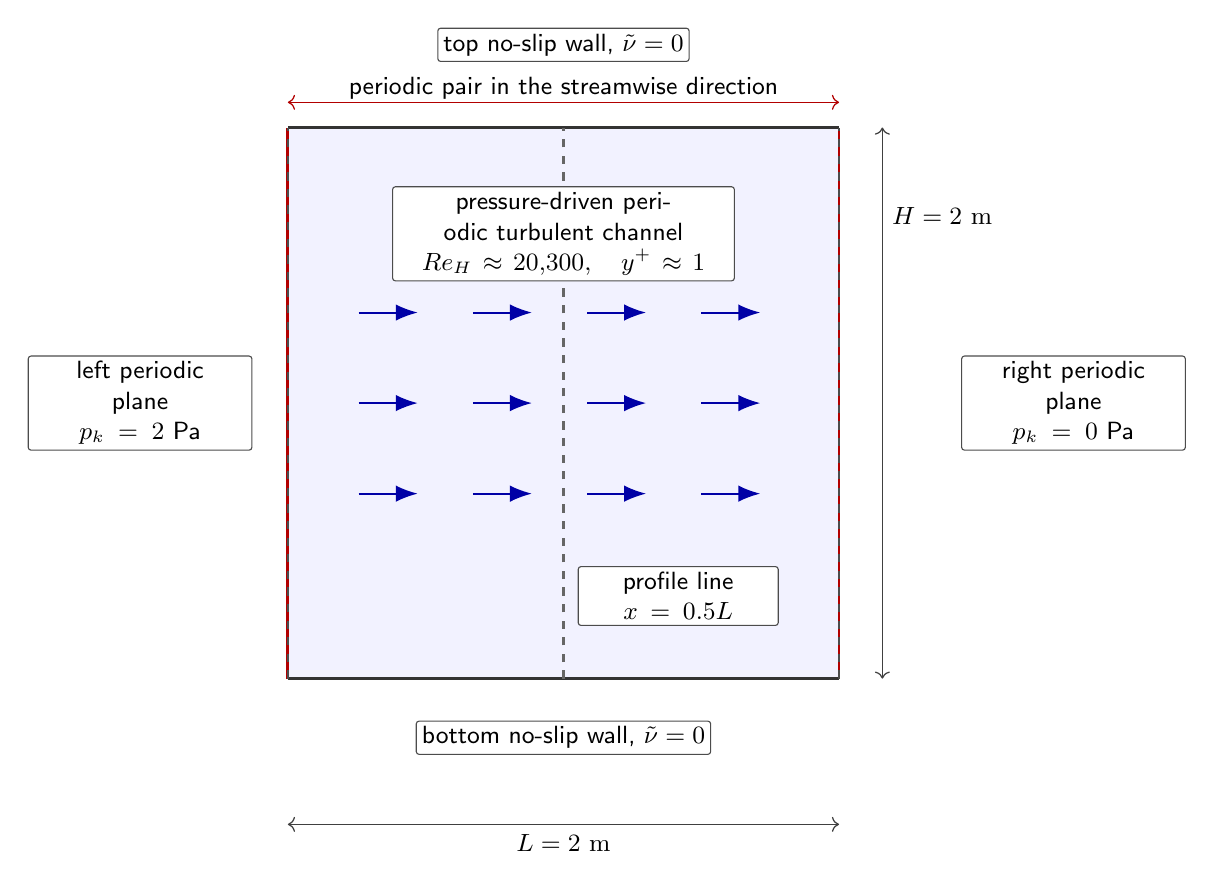
\begin{tikzpicture}[
  font=\sffamily\small,
  flow/.style={-{Latex[length=2.8mm]}, line width=0.7pt, draw=blue!65!black},
  dim/.style={<->, line width=0.45pt, draw=black!75},
  wall/.style={line width=1.1pt, draw=black!80},
  bc/.style={draw=black!70, fill=white, rounded corners=1pt, inner sep=2pt, align=center}
]

\def\L{7}
\def\H{7}

\fill[blue!5] (0,0) rectangle (\L,\H);
\draw[wall] (0,0) -- (\L,0);
\draw[wall] (0,\H) -- (\L,\H);
\draw[red!70!black, line width=1.0pt] (0,0) -- (0,\H);
\draw[red!70!black, line width=1.0pt] (\L,0) -- (\L,\H);
\draw[black!70, dashed, line width=0.75pt] (0,0) -- (0,\H);
\draw[black!70, dashed, line width=0.75pt] (\L,0) -- (\L,\H);

\foreach \y in {2.35,3.50,4.65} {
  \foreach \x in {0.90,2.35,3.80,5.25} {
    \draw[flow] (\x,\y) -- ++(0.75,0);
  }
}

\node[bc, anchor=east, text width=27mm] at (-0.45,0.5*\H) {left periodic\\plane\\$p_k=2$ Pa};
\node[bc, anchor=west, text width=27mm] at (\L+1.55,0.5*\H) {right periodic\\plane\\$p_k=0$ Pa};

\node[bc] at (0.5*\L,\H+1.05) {top no-slip wall, $\tilde{\nu}=0$};
\node[bc] at (0.5*\L,-0.75) {bottom no-slip wall, $\tilde{\nu}=0$};
\draw[<->, line width=0.45pt, draw=red!70!black] (0,\H+0.32) -- node[above, fill=white, inner sep=1pt] {periodic pair in the streamwise direction} (\L,\H+0.32);

\draw[black!60, dashed, line width=0.8pt] (0.5*\L,0) -- (0.5*\L,\H);
\node[bc, anchor=west, text width=24mm] at (0.5*\L+0.18,1.05) {profile line\\$x=0.5L$};

\draw[dim] (0,-1.85) -- node[below] {$L=2~\mathrm{m}$} (\L,-1.85);
\draw[dim] (\L+0.55,0) -- node[pos=0.84, right] {$H=2~\mathrm{m}$} (\L+0.55,\H);

\node[bc, text width=42mm] at (0.5*\L,5.65) {pressure-driven periodic turbulent channel\\$Re_H\approx 20{,}300,\quad y^+\approx 1$};

\end{tikzpicture}
\end{document}
